% !TeX spellcheck = sl_SI

\chapter{Zasnova metamateriala}\label{sec:Zasnova_metamateriala}

    Z definiranimi pogoji dimenzioniranja v poglavju \ref{sec:ROC_statika} in z znanimi materialnimi lastnostmi modula elastičnosti $E$ in gostote $\rho$ pridobljenimi v poglavju \ref{sec:PLA}, lahko zasnujemo in z MKE (poglavje \ref{sec:MKE}) ovrednotimo dejanski primer reprezentativne osnovne celice (ROC), ki izkazuje kvazi ničelno togost (KNT). Nato znano ROC vpeljemo v poglavje \ref{sec:dinamika_metamaterialnega_vibroizolatorja} in jo tvorimo v metamaterialno (MM) verigo, ki izkazuje lastnost pasovno zavrnitvenega filtra (PZF). Analitično verigo neskončnih členov aproksimiramo z zaporedjem desetih ROC-jev in dinamični sistem rešimo numerično. 

    \section{Zasnova in numerično vrednotenje ROC}

        Uporabimo končno enačbo (\ref{eq:kp}) pozitivne togosti poglavja \ref{sec:Izpeljava_elementa_s_pozitivno_togostjo} in enačbe (\ref{eq:kn}) negativnih togosti ter ob združitvenih pogojih (\ref{eq:k1k2k3}) za KNT dobimo dimenzijske enačbe ROC. Upoštevamo eksperimentalno pridobljen $E$ pri sobni temperaturi. Odločimo se za pravokotni prerez ROC-ja, kar vodi v vztrajnostni moment ploskve: 
        \begin{equation}
            I_1=\frac{b\, t_1^3}{l_1} \, , \,\,\,\,\,\,\,\,\,\,\,\,\,\,\,\, I_2=\frac{b\, t_2^3}{l_2} \,.
        \end{equation}
        Tako dobimo dimenzije ROC na sliki \ref{fig:ROC_dimenzija}.
        \begin{figure}[!hb]
            \centering
            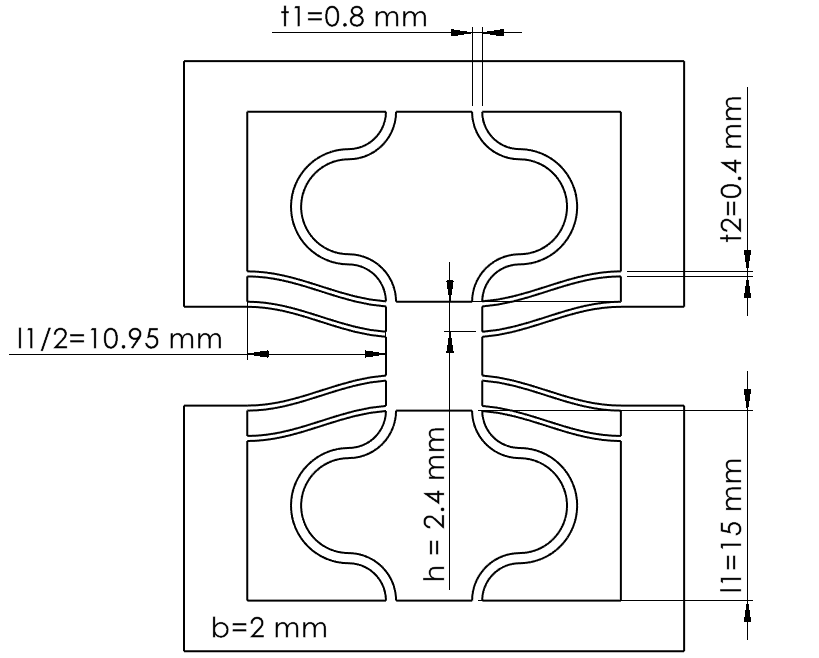
\includegraphics[width=0.51\textwidth]{Magisterski praktikum/slike/metodologija/ROC_dimenzije.png}
            \caption{Skica ROC-ja z vsemi dimenzijami.}\label{fig:ROC_dimenzija}
        \end{figure}
        
        
        
        
        Vredno omembe je povečan osrednji del za zagotovitev dovolj prostora za deformacijo in hkrati večjo resonančno maso $m$. Pomembno je tudi izpostaviti, da smo omejeni na minimalno dimenzijo šobe 3D tiskalnika, kar znaša $0,4$ mm. Torej so vse končne dimenzije faktor tega števila. 

        Za MKE analizo smo uporabili ANSYS \textit{Mechanical}. Za izvajanje statične nelinearne analize uporabimo paket, ki je namenjen analizi mehanskih struktur (slika \ref{fig:MKE_statika}). Za uporabljenim paketom stoji Ansysov skriptni jezik APDL (\textit{ang. Ansys Parametric Design Language}). Jezik nudi parameterizacijo, izvajanje logičnih funkcij in drugih kompleksnih matematičnih operacij, kar vodi v efektivni komercialni program za reševanje po MKE \cite{thompson2017ansys}. 
        
        Predpostavili smo lupino in pomrežili z 4902 elementi preko 5720 vozlišč z tipom elementa SHELL181. Vpeljali smo tudi materialni model GPLA-ja glede na meritve. 
        
        \begin{figure}[!hb]
            \centering
            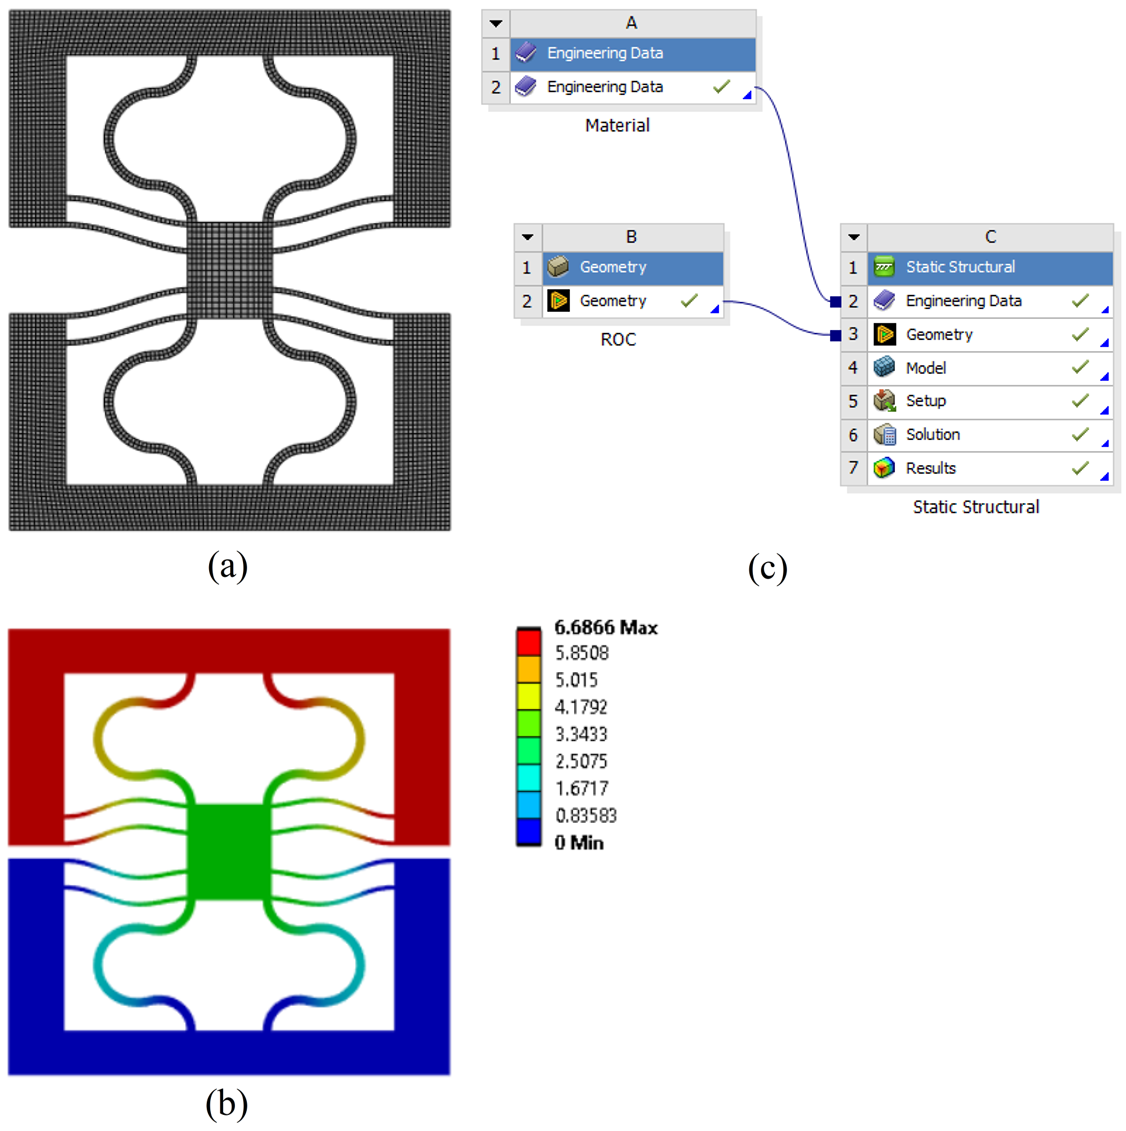
\includegraphics[trim={0.0cm 0.0cm 0.0cm -2.0cm}, clip, width=0.8\textwidth]{Magisterski praktikum/slike/metodologija/MKE_statika.png}
            \caption{(a) Pomrežen model ROC-ja, (b) njegova deformirana lega z prikazano deformacijo in (c) ANSYS \textit{Workbench} shema simulacije.}\label{fig:MKE_statika}
        \end{figure}

        \newpage
        Dimenzionirano osnovno celico lahko vrednotimo z grafom sile-pomika $F$-$X$ na \ref{fig:sile_ROC} in pri tem uporabimo analitične enačbe dimenzionirana omenjene v uvodu tega poglavja, zvezno definicijo sile ROC $F_{\text{ROC}}(X)$ v enačbi \ref{eq:F-ROC} in MKE model zgoraj. 
        
        \begin{figure}[!hb]
            \centering
            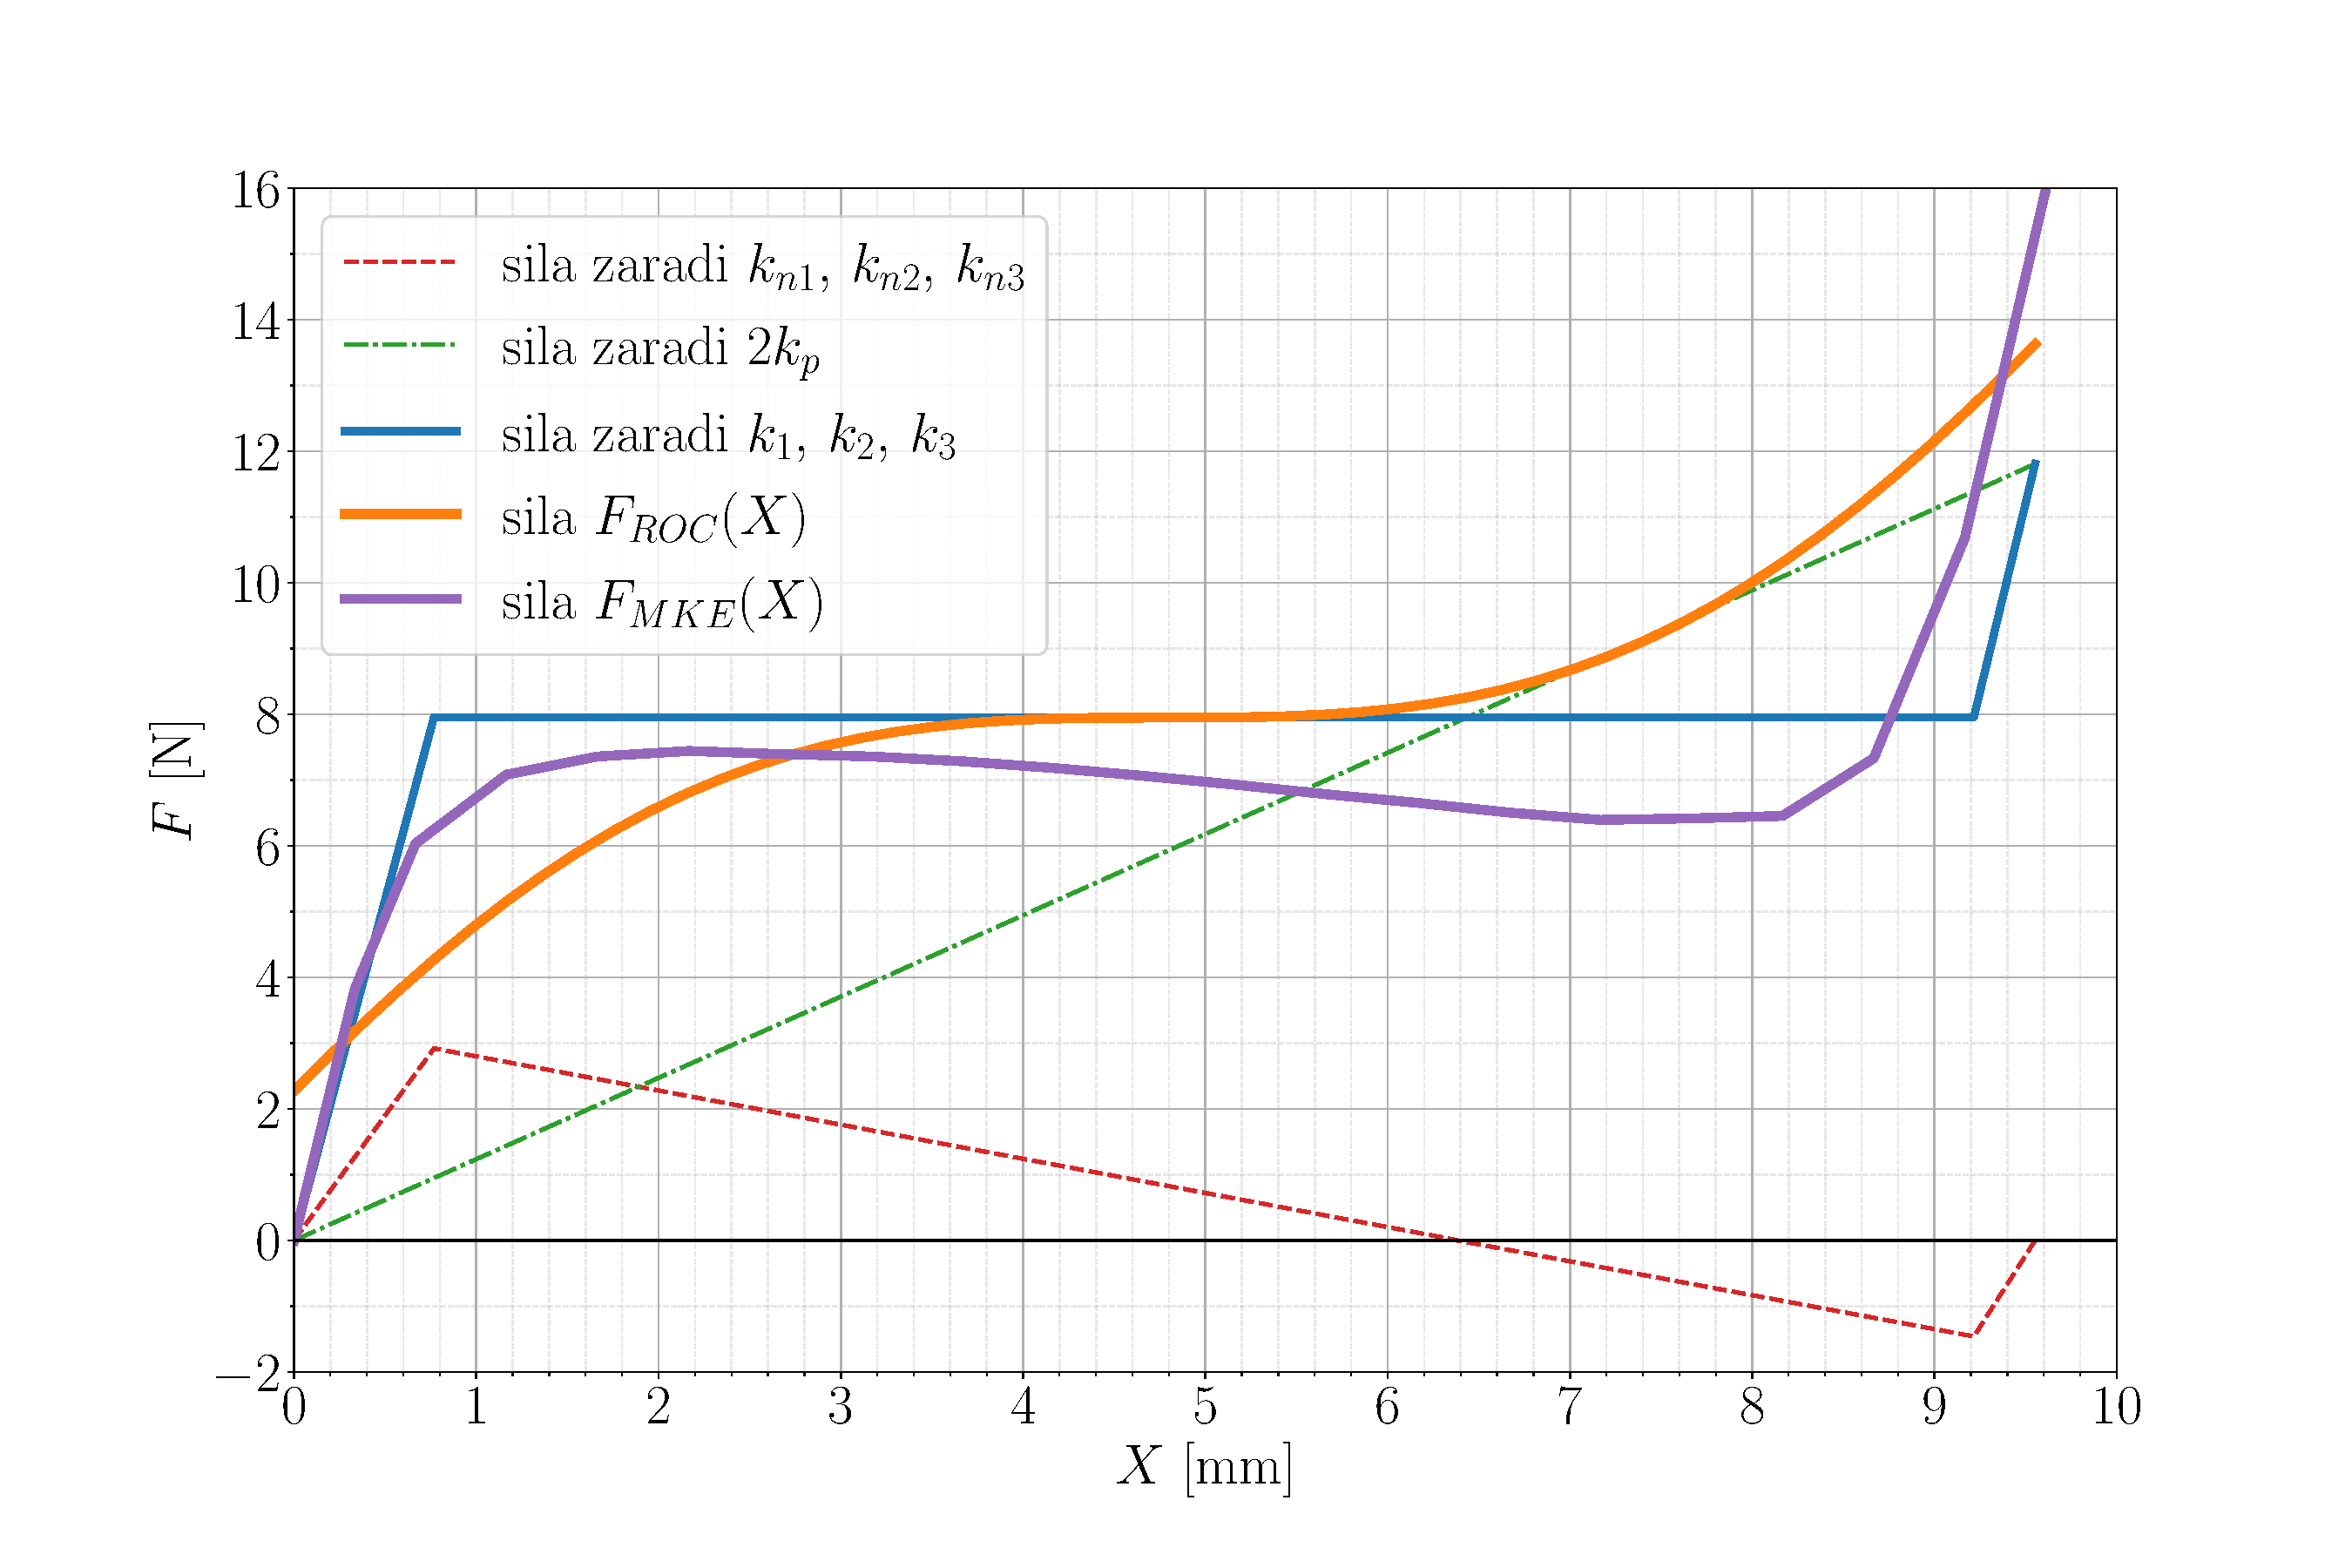
\includegraphics[trim={2.0cm -1.0cm 2.0cm -2.0cm}, clip, width=1\textwidth]{Magisterski praktikum/slike/metodologija/sile_ROC.pdf}
            \caption{Analitične in numerične primerjave poteka $F$-$X$ ROC-ja.}\label{fig:sile_ROC}
        \end{figure}

        Vidimo lahko, da je analitična sila po Taylorjevi vrsti $F_{ROC}(X)$ približek diskrezno izpeljane sile zaradi togosti $k_1$, $k_2$ in $k_3$. 
        Numerični potek sile $F_{MKE}(X)$ po MKE modelu je prav tako blizu analitično določeni sili. 

        V naslednjem koraku lahko z določenimi lastnostmi togosti zasnujemo metamaterialno (MM) verigo in ovrednotimo njeno dinamiko.

    \newpage
    \section{Zasnova in numerično vrednotenje MM verige}\label{sec:zasnova_MM_verige}
        
        V naslednjem koraku grafično prikažemo enačbo disperzijske krivulje (\ref{eq:disperzijska_krivulja}) za konkretni primer metamateriala $n$-tih ROC-jev zasnovanih v prejšnjem poglavju. Preko znane geometrije in znane gostote $\rho_{GPLA}$ lahko določimo maso ROC-ja $M=1,766\text{ g}$ in maso resonatorja $m=0,145\text{ g}$. Tako lahko določimo vse brezdimenzijske vrednosti na podlagi poglavja \ref{sec:dinamika_metamaterialnega_vibroizolatorja}. 
        Določimo amplitudi $A=7$ in $B=0,007$, ter brezdimenzijsko maso $\beta = m/M = 0,082$. V grafu \ref{fig:FRF_disperzijska} prikažemo disperzijske krivulje za različne vrednosti brezdimenzijske togosti $\alpha$ in dušenja $\zeta$. Tam kjer je $\Im(\mu_u)<1$ je prenosnost vibracij zmanjšana in je prisotna pasovna vrzel. Vidimo, da je pasovna vrzel za nizko togost $k$ pri zelo nizkih frekvencah.
        \begin{figure}[!hb]
            \centering
            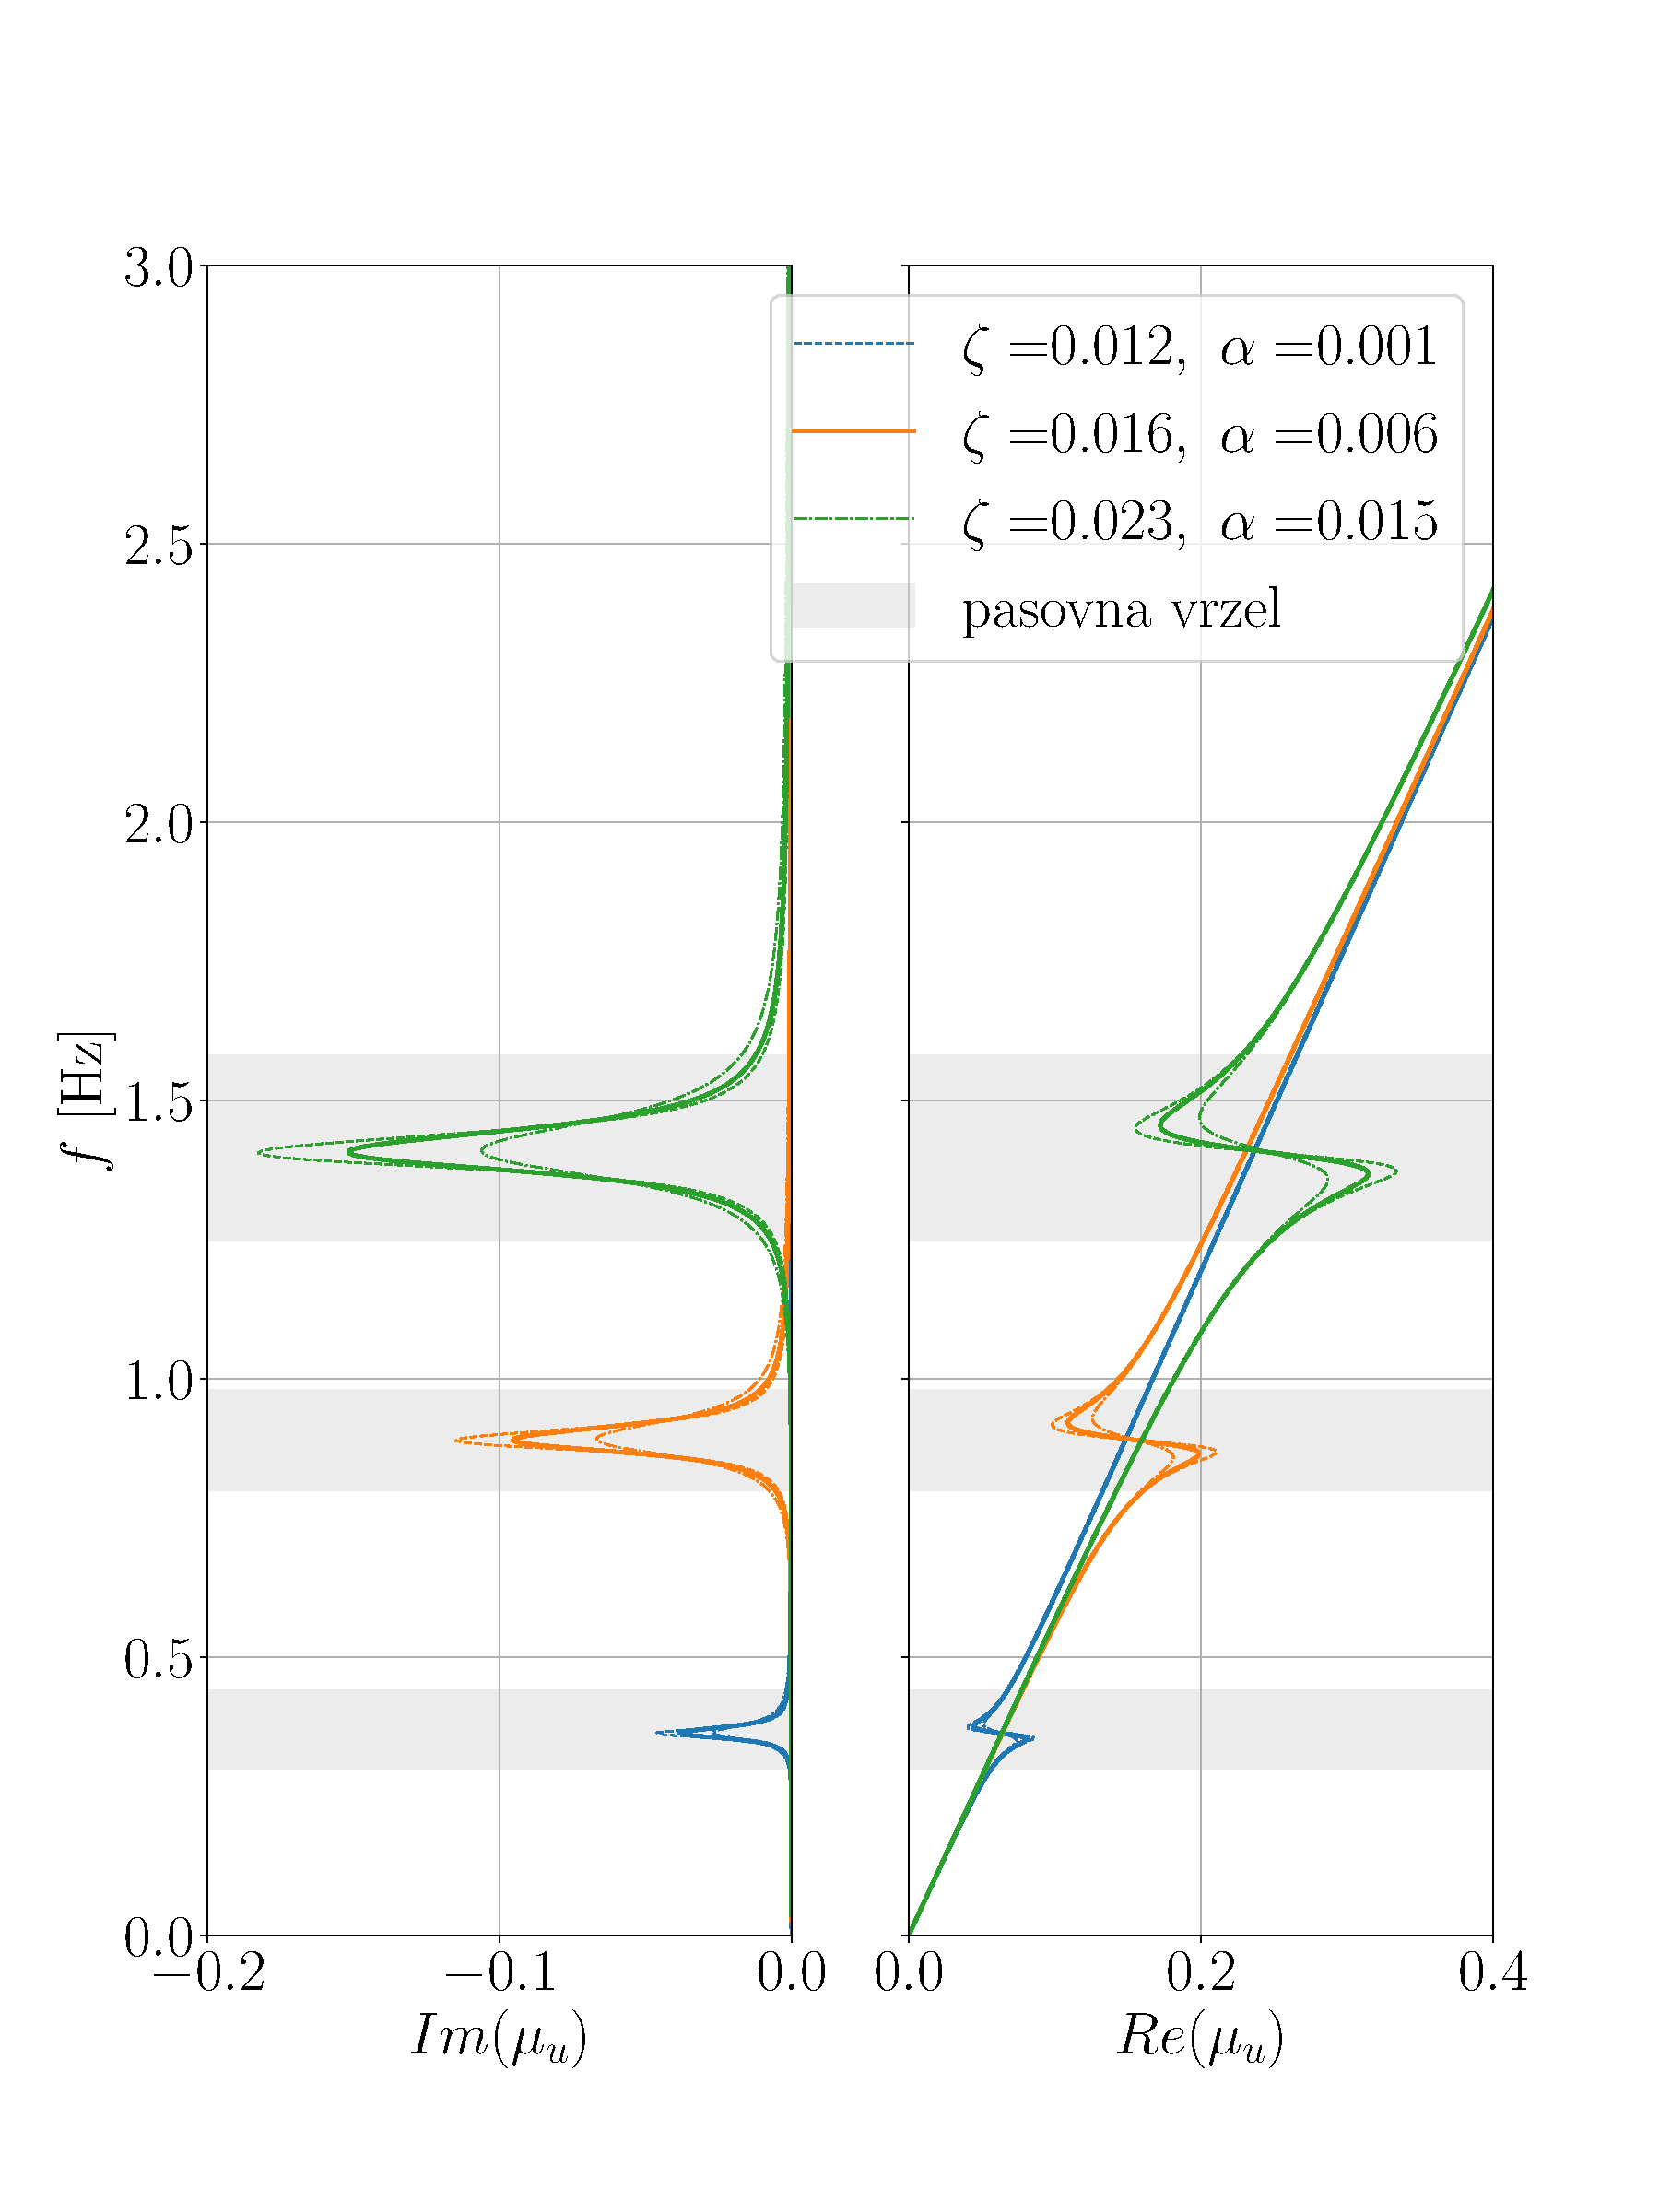
\includegraphics[trim={0.0cm 0.0cm 0.0cm 3.0cm}, clip, width=0.8\textwidth]{Magisterski praktikum/slike/metodologija/FRF_disperzijska.pdf}
            \caption{Disperzijska krivulja $\mu(f)$.}\label{fig:FRF_disperzijska}
        \end{figure} 
        
        \newpage
        Iz zasnovane ROC tvorimo enodimenzionalno verigo $n=10$ ROC-jev oziroma naš metamaterial (MM), ki je viden na sliki \ref{fig:MM_veriga_2}. Prva vzmet s togostjo $K=2 k_p$ je fiksno pritrjena na podlago, zadnja vzmet in tako tudi zadnja masa $M$ je prosta. Prvi ROC v verigi je harmonično vzbujen pri različnih frekvencah $f$. 
        
        Izpeljemo gibalno enačbo sistema: 
        \begin{equation}\label{eq:gibalna_enacba_MM}
            [M] \ddot{\vv{X}}(t)+[C] \dot{\vv{X}}(t)+[K] \vv{X}(t)=\vv{F}(t) \, ,
        \end{equation}
        kjer je $\vv X=\left[\begin{array}{lllllll}U_1 & Q_1 & U_2 & Q_2 & \cdots & U_n & Q_n\end{array}\right]^T$ vektor pomikov $U_j$ primarnih mas in relativnih pomikov $Q_j$ med primarno in resonančno maso za $j=1, ..., n$. Masne $[M]$, dušilne $[C]$ in togostne $[K]$ matrike so podane kot: 
        \begin{equation}
            [M]=\left[\begin{array}{ccccccc}
            M & 0 & 0 & 0 & \cdots & 0 & 0 \\
            m & m & 0 & 0 & \cdots & 0 & 0 \\
            0 & 0 & M & 0 & \cdots & 0 & 0 \\
            0 & 0 & m & m & \cdots & 0 & 0 \\
            \vdots & \vdots & \vdots & \vdots & \ddots & \vdots & \vdots \\
            0 & 0 & 0 & 0 & \cdots & M & 0 \\
            0 & 0 & 0 & 0 & \cdots & m & m
            \end{array}\right]\,,
        \end{equation}
        \begin{equation}
            [C]=\left[\begin{array}{ccccccc}
            0 & -c & 0 & 0 & \cdots & 0 & 0 \\
            0 & c & 0 & 0 & \cdots & 0 & 0 \\
            0 & 0 & 0 & -c & \cdots & 0 & 0 \\
            0 & 0 & 0 & c & \cdots & 0 & 0 \\
            \vdots & \vdots & \vdots & \vdots & \ddots & \vdots & \vdots \\
            0 & 0 & 0 & 0 & \cdots & 0 & -c \\
            0 & 0 & 0 & 0 & \cdots & 0 & c
            \end{array}\right]\,,
        \end{equation}
        \begin{equation}
            [K(Q_j)]=\left[\begin{array}{cccccccccccc}
            2 K & -k & -K & 0 & 0 & \cdots & 0 & 0 & 0 & 0 & 0 & 0 \\
            0 & k & 0 & 0 & 0 & \cdots & 0 & 0 & 0 & 0 & 0 & 0 \\
            -K & 0 & 2 K & -k & -K & \cdots & 0 & 0 & 0 & 0 & 0 & 0 \\
            0 & 0 & 0 & k & 0 & \cdots & 0 & 0 & 0 & 0 & 0 & 0 \\
            \vdots & \vdots & \vdots & \vdots & \vdots & \ddots & \vdots & \vdots & \vdots & \vdots & \vdots & \vdots \\
            0 & 0 & 0 & 0 & 0 & \cdots & -K & 0 & 2 K & -k & -K & 0 \\
            0 & 0 & 0 & 0 & 0 & \cdots & 0 & 0 & 0 & k & 0 & 0 \\
            0 & 0 & 0 & 0 & 0 & \cdots & 0 & 0 & -K & 0 & K & -k \\
            0 & 0 & 0 & 0 & 0 & \cdots & 0 & 0 & 0 & 0 & 0 & k
            \end{array}\right]
        \end{equation}

        in je $k=F_{\text{ROC}}'(Q_j)$ nelinearna togost. 
        
        Vektor sile je podan kot $\vv{F}=\left[\begin{array}{llll}f \sin (2\pi f t) & 0 & \cdots & 0\end{array}\right]^T$.

        \newpage
        \begin{figure}[!hb]
            \centering
            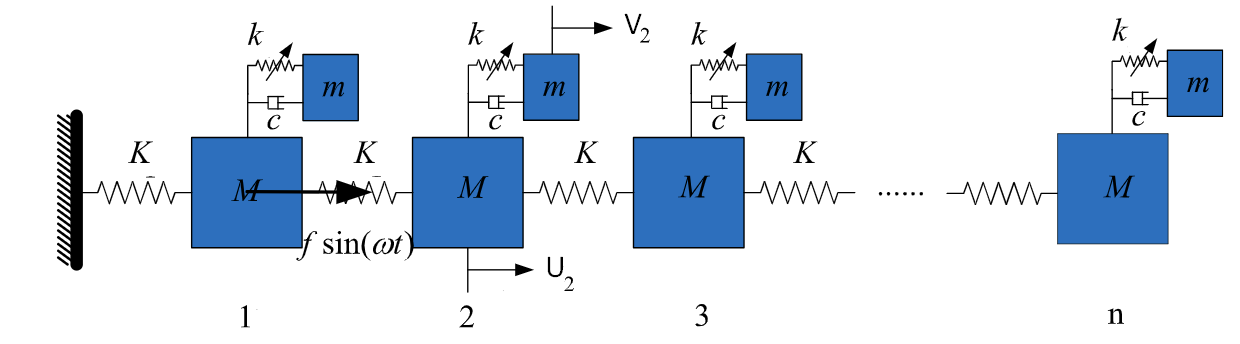
\includegraphics[scale=0.59]{slike/metodologija/MM_veriga_2.png}
            \caption{Enodimenzionalna metamaterialna veriga z robnimi pogoji.}\label{fig:MM_veriga_2}
        \end{figure}

        na spodnji sliki \ref{fig:MM_veriga_MKE} vidimo, da je dinamska numerična analiza narejena na statično predobremenjenem MM. Predobremenitev je enaka statični masi, ki jo želimo vibroizolirati. 

        \begin{figure}[!hb]
            \centering
            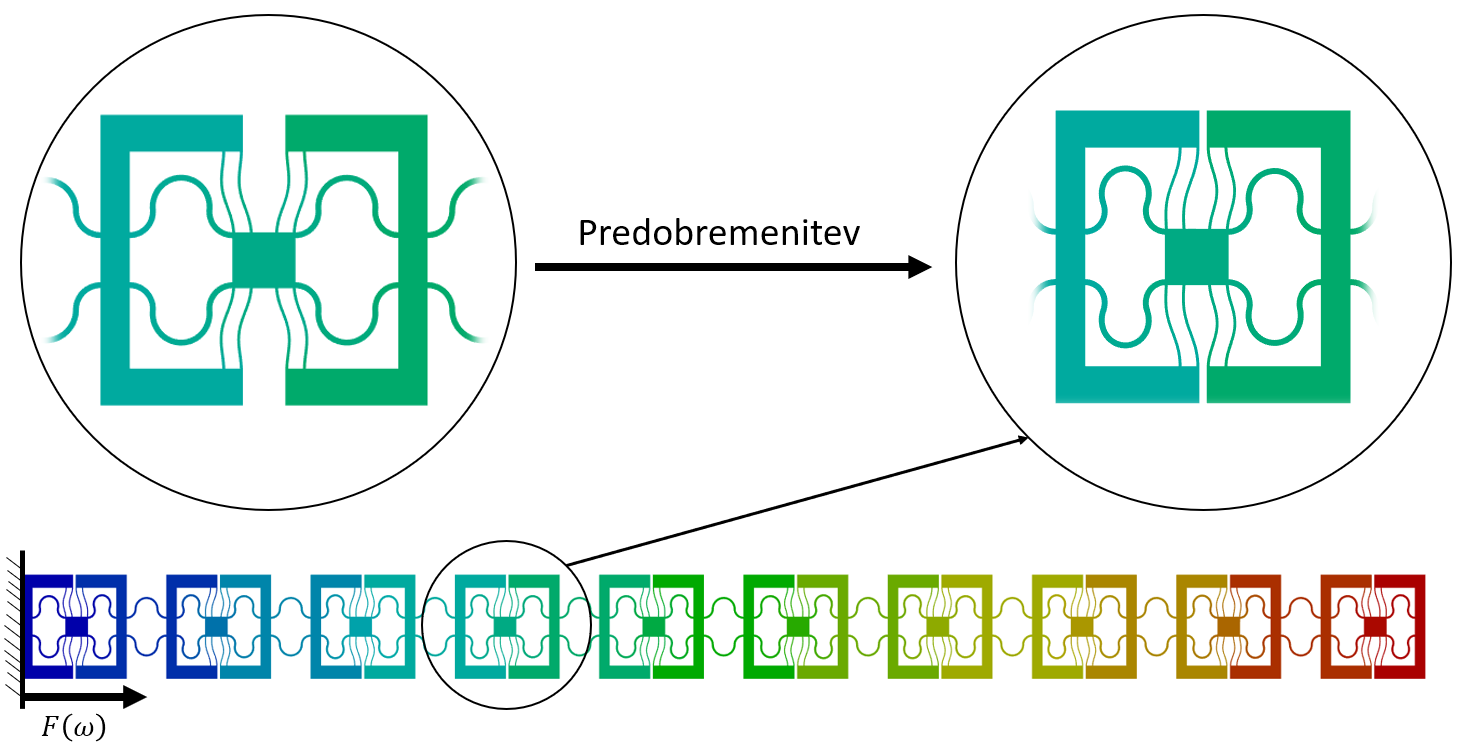
\includegraphics[trim={0.0cm 0.0cm 0.0cm 0.0cm}, clip, width=1.0\textwidth]{Magisterski praktikum/slike/metodologija/ROC_MKE_veriga.png}
            \caption{MM veriga z $n=10$ pri čemer je vidna predobremenitev.}\label{fig:MM_veriga_MKE}
        \end{figure}

        Problem lahko rešimo direktno z numeričnim reševanjem diferencialne enačbe pri začetnih pogojih $\vv X = \dot{\vv{X}}=\vv 0$ z uporabo implicitne Runge-Kutta sheme. Časovno integriramo pri različnih frekvencah $f$, in v frekvenčni domeni preko Fouriereve transformacije pogledamo prenosljivost $T_{\text{R-K}}$, ki je razmerje med pomikom zadnje glavne mase $U_n$ in prve mase $U_1$. 

        Indirektno lahko homogeni del gibalne enačbe (\ref{eq:gibalna_enacba_MM}) rešimo brez integriranja z linearizacijo togosti \cite{rao2017mechanical}. Če predpostavimo, da imamo dovolj majhne pomike lahko za $k\approx 0$ določimo prenosno funkcijo $T_{\text{lin}}$ z uporabo pseudoinverza:
        \begin{align}
            -\vv{X}= \left\{ [K]+ i \, \omega [D]-\omega^2 [M] \right\}^{-1} \vv{F}\,.
        \end{align}

        V sledečem poglavju si ogledamo prenosno funkcijo $T(f)$ kot končen rezultat. 

